\documentclass[xcolor={dvipsnames},aspectratio=169]{beamer}
\usetheme{eth}
\usepackage{graphicx}
\graphicspath{ {img/} }
\usepackage{datetime2}
\usepackage{siunitx}
\usepackage{amsmath}
\usepackage{subcaption}
\usepackage{amssymb}
\usepackage{tabularx}
\newcolumntype{L}{>{\centering\arraybackslash}m{2cm}}
\usepackage{rotating}
\usepackage{multicol}
\usepackage{multirow}
\usepackage{booktabs}
\usepackage{movie15}
\usepackage{mhchem}
\usepackage{hyperref}
\usepackage{animate}
\usepackage{pgfplots}
\pgfdeclarelayer{bg}    % declare background layer
\pgfsetlayers{bg,main}  % set the order of the layers (main is the standard layer)
\usepackage{tikz}
\usetikzlibrary{dsp, arrows, positioning, chains, fit, calc, patterns}
\usepackage[american]{circuitikz}
\usepackage[electronic]{ifsym}
\usepackage[dvipsnames]{xcolor}
\usepackage{pifont}% http://ctan.org/pkg/pifont
\newcommand{\cmark}{\textcolor{ForestGreen}{\ding{51}}}
\newcommand{\xmark}{\textcolor{BrickRed}{\ding{55}}}

\colorlet{titlefgcolor}{ETHBlue}
\colorlet{accentcolor}{ETHGreen}

\setbeamertemplate{footline}
{%
  \leavevmode%
  \hbox{\begin{beamercolorbox}[wd=.5\paperwidth,ht=2.5ex,dp=1.125ex,leftskip=.3cm plus1fill,rightskip=.3cm]{author in head/foot}%
  \usebeamerfont{author in head/foot}\insertshortauthor
    
  \end{beamercolorbox}%
  \begin{beamercolorbox}[wd=.38\paperwidth,ht=2.5ex,dp=1.125ex,leftskip=.3cm,rightskip=.3cm plus1fill]{title in head/foot}%
  \usebeamerfont{title in head/foot}\insertshorttitle
    
  \end{beamercolorbox}%
  \begin{beamercolorbox}[wd=.12\paperwidth,ht=2.5ex,dp=1.125ex,center]{author in head/foot}%
    \usebeamerfont{author in head/foot} \insertframenumber{} / \inserttotalframenumber
  \end{beamercolorbox}}%
  \vskip0pt%
}

\newenvironment<>{stfblock}[1]{%
  \setbeamercolor{block title}{fg=white,bg=OliveGreen}%
  \begin{block}#2{#1}}{\end{block}}
\newenvironment<>{ntfblock}[1]{%
  \setbeamercolor{block title}{fg=white,bg=RedOrange}%
  \begin{block}#2{#1}}{\end{block}}
  
\DeclareMathOperator{\Tr}{Tr}
\DeclareMathOperator{\Diag}{diag}

\title{Helical Auxetic Yarn Modelling}
\subtitle{}
\author{Brett Hannigan \\
	\texttt{brett.hannigan@hest.ethz.ch}
}
\institute{Biomedical and Mobile Health Technology (BMHT) Lab}
\date{2022-11-22}

\begin{document}

\colorlet{titlebgcolor}{ETHGreen}
\def\titlefigure{}
\setlength{\titleboxwidth}{0.75\textwidth}			% Change box width
%\title{Weekly Updates -- Fall 2021}
\titleframe

\frame
{
	\frametitle{Helical Auxetic Sensors}
	\begin{columns}
		\begin{column}{0.5\textwidth}
			\begin{figure}
				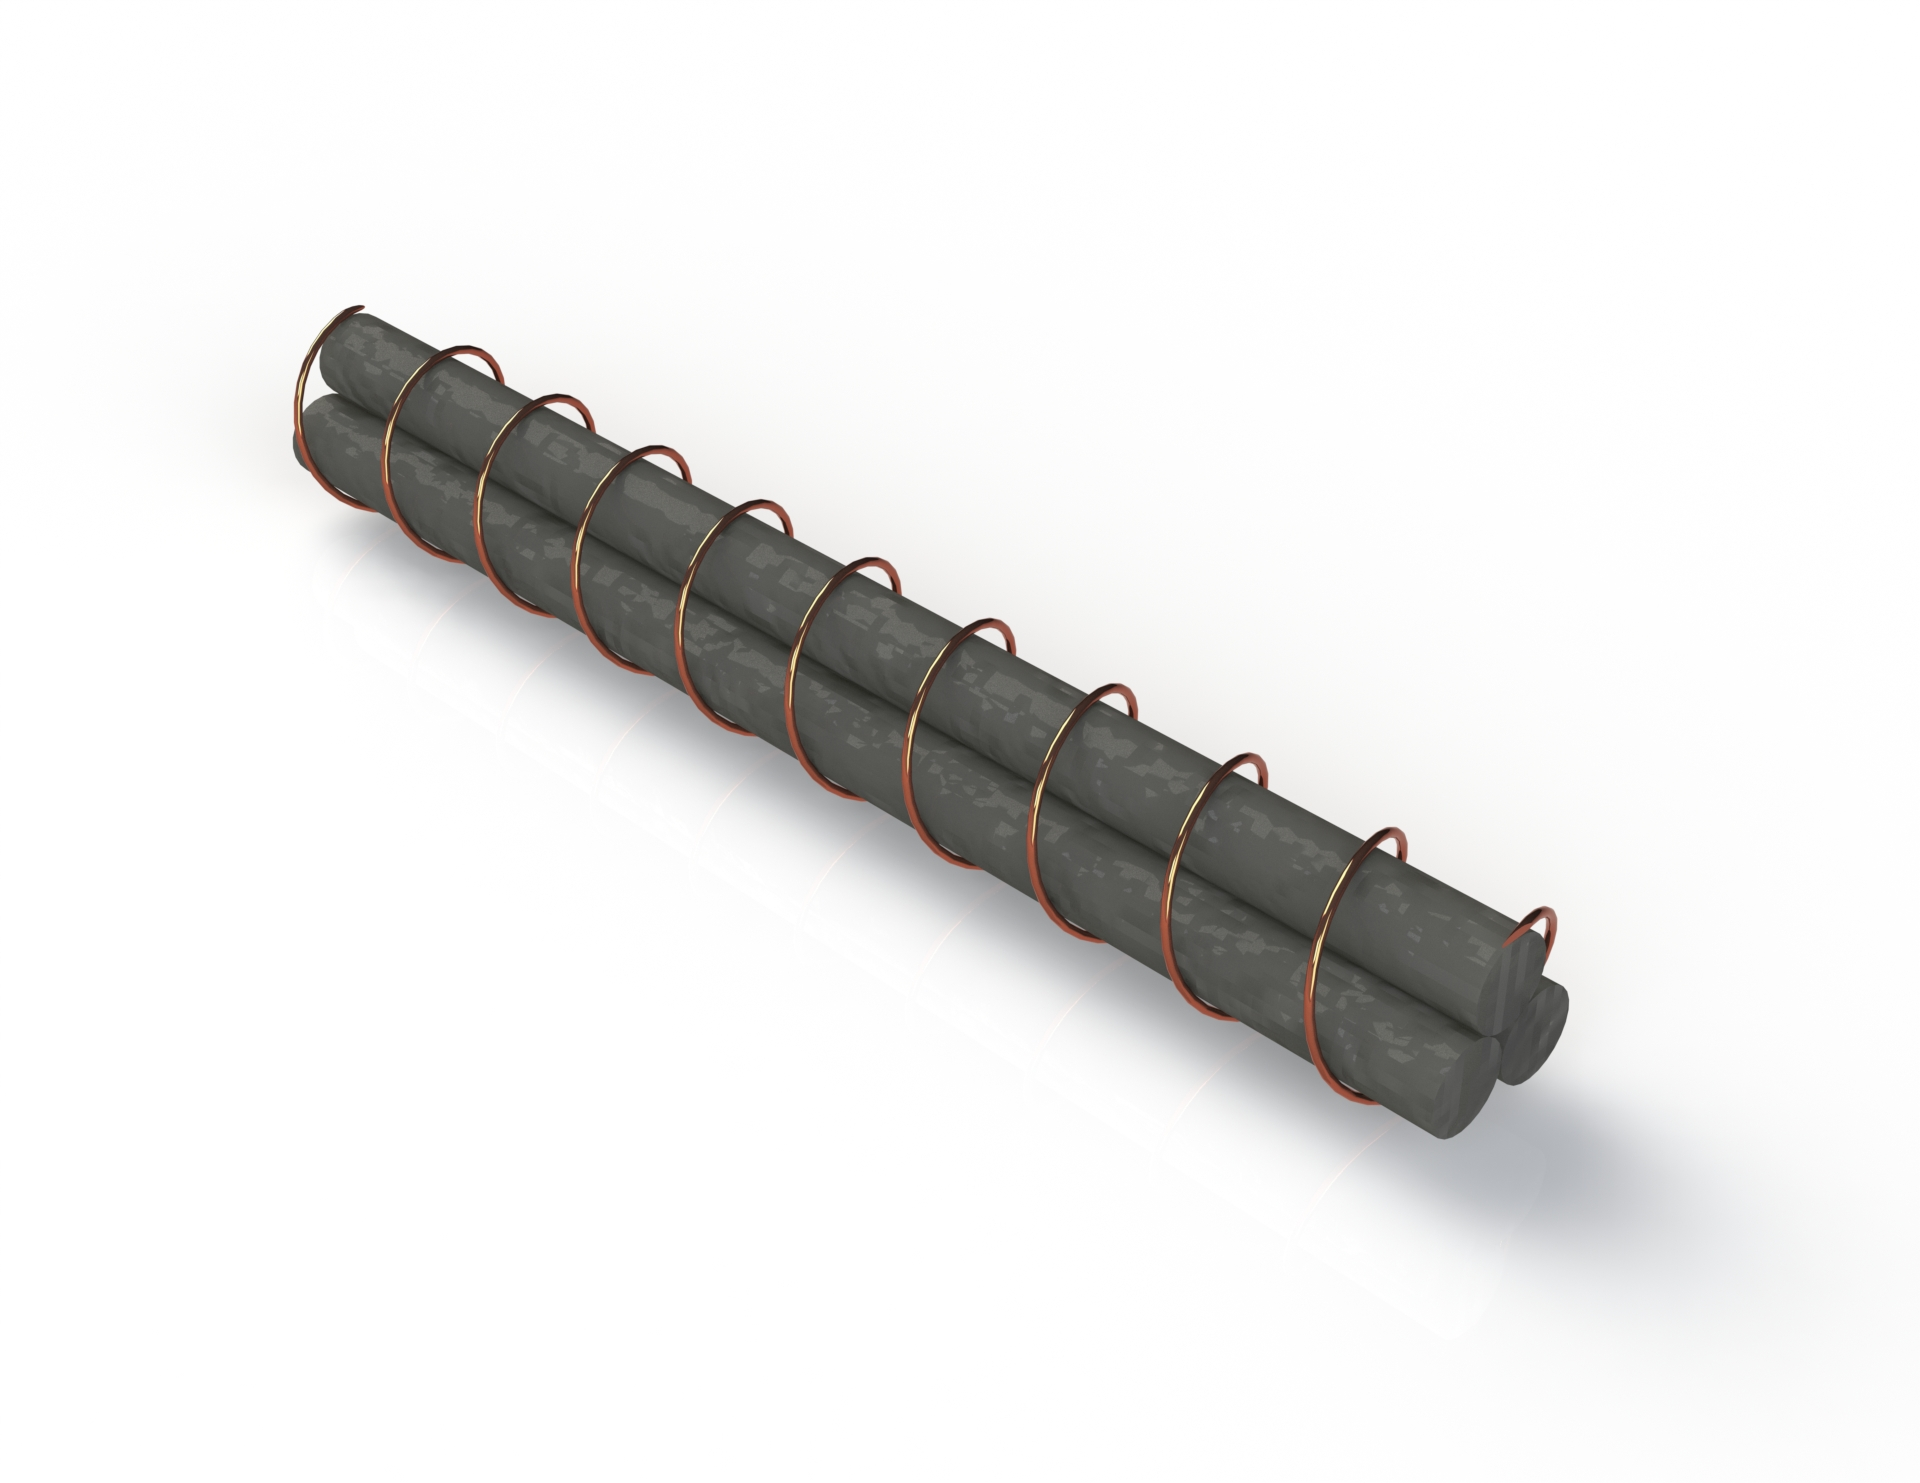
\includegraphics[width=0.6\textwidth]{AuxeticSensor_Unstretched_Shadow}
				\caption{Unstretched state}
			\end{figure}
		\end{column}
		\begin{column}{0.5\textwidth}
			\begin{figure}
				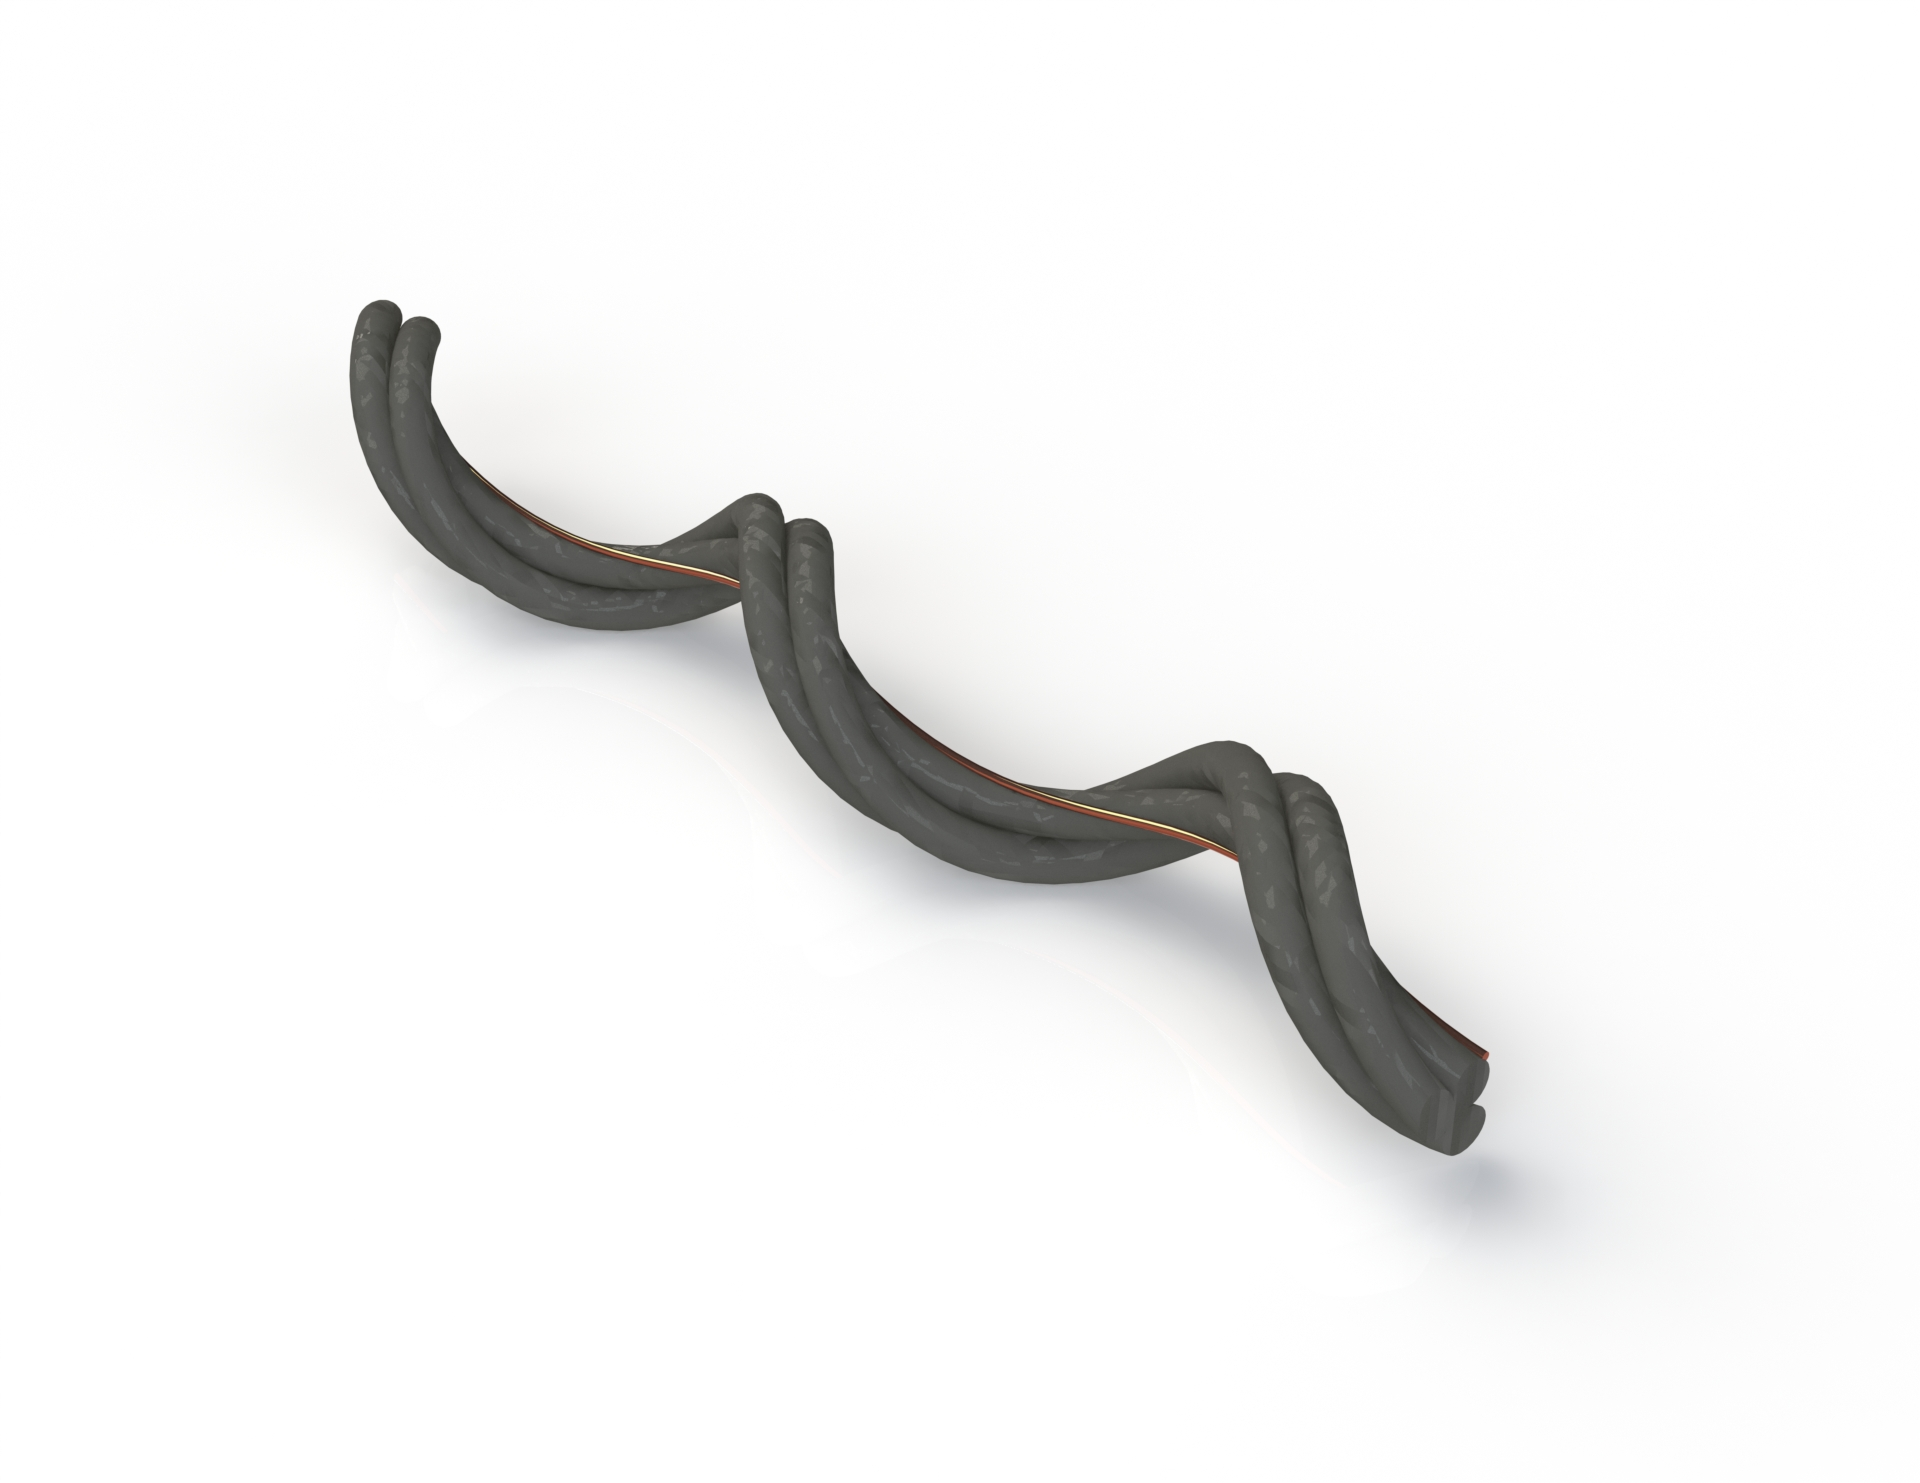
\includegraphics[width=0.6\textwidth]{AuxeticSensor_Stretched_Shadow}
				\caption{Stretched state}
			\end{figure}
		\end{column}
	\end{columns}
	\begin{itemize}
		\item Want a model to determine exact geometry at arbitrary strain.
		\item Parameters:
		\begin{itemize}
			\item Stretchable elastic fibre (initially core) with circular cross-section, initial diameter $d_{e}(\varepsilon=0)$, length $l_0$, and Poisson's ratio $\nu$.
			\item Perfectly inelastic wire (initially winding) with circular cross-section, diameter $d_w$, $n$ turns, and pitch $p_0=\frac{l_0}{n}$.
		\end{itemize}
		\item Use model to calculate capacitance?
	\end{itemize}
}

\frame
{
	\frametitle{Approach to Modelling}
	Approach:
	\begin{enumerate}
		\item Obtain equation for a helical coil in space.
		\item Determine the constraints that link the geometry of the elastic and inelastic fibres w.r.t. overall sensor strain.
		\item Slice the geometry with a plane along the sensor axis to get the cross-section.
		\item Compute capacitance computationally from the 2-D cross-section geometry.
	\end{enumerate}
	Assumptions:
	\begin{itemize}
		\item Elastic and stiff fibres are concentric.
		\item The wire helix geometry is independent of the elastic element.
		\item The elastic fibre is stiff and it does not comply to the wire (maintains a circular cross-section along the helical path, with point contact).
		\item Capactiance may be calculated from the cross-section, integrated along the sensor (i.e., no self-capacitance between coils).
	\end{itemize}
}

\frame
{
	\frametitle{Helical Curve}
	\begin{itemize}
		\item Begin with the equation for a helical path in space parameterized by $t$.
		\item Helix will run along the x-axis with radius $r_M$ and pitch $p$.  
	\end{itemize}
	\begin{columns}
		\begin{column}{0.5\textwidth}
			\begin{block}{Equation for a helical path}
				\begin{equation}
					\vec{h}(t) =
					\begin{cases}
						x(t) &= \frac{p}{2\pi}t \\
						y(t) &= r_M\cos(t) \\
						z(t) &= r_M\sin(t)
					\end{cases} \label{eq:helix}
				\end{equation}
			\end{block}
		\end{column}
		\begin{column}{0.5\textwidth}
			\begin{figure}
				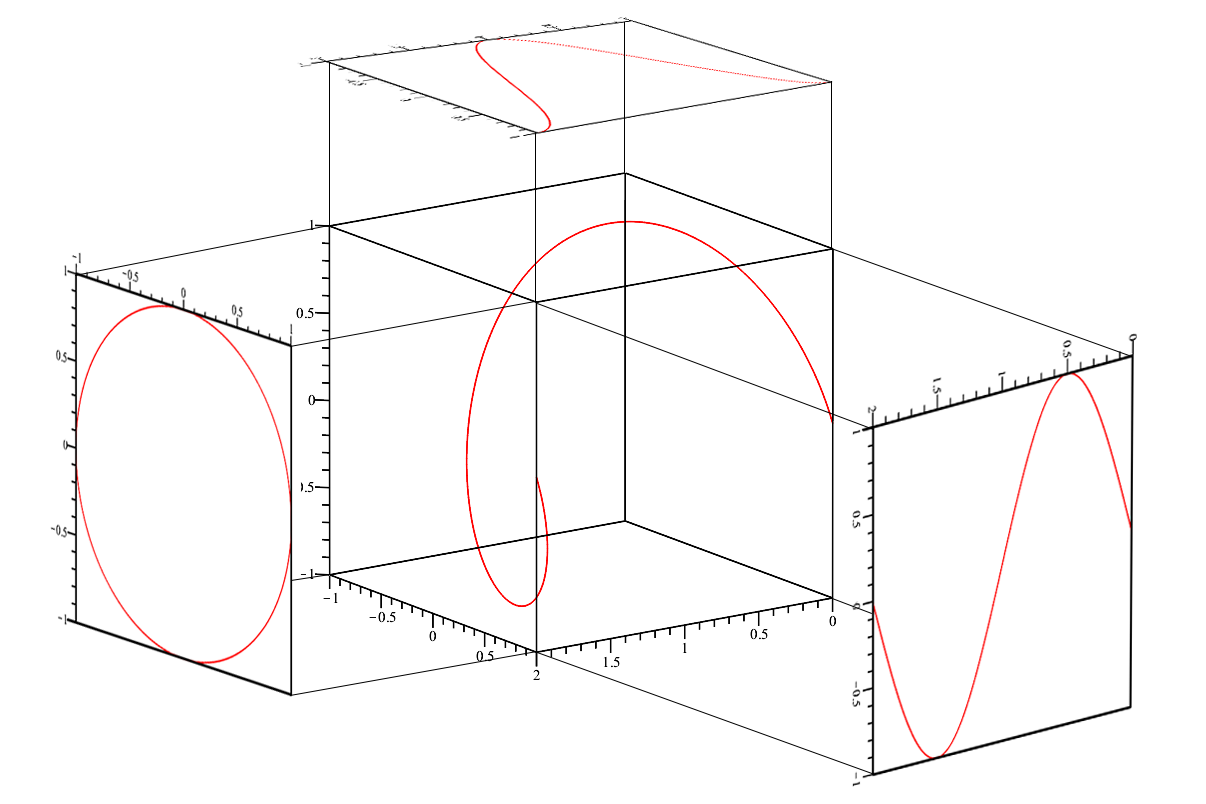
\includegraphics[width=\textwidth]{HelicalPath}
			\end{figure}
		\end{column}
	\end{columns}
}

\frame
{
	\frametitle{Helical Coil with Volume: Coordinate Set-Up\footnotemark}
	\begin{itemize}
		\item Need to add thickness to the helix by tracing its path with a circular cross-section.
		\item We require an orthonormal basis coordinate system $\{\vec{p}(t), \vec{q}(t), \vec{r}(t)\}$ for this circle, where:
		\begin{itemize}
			\item \textcolor{red}{$\vec{p}(t)$} is tangent to the helical path at point $\vec{h}(t)$
			\item \textcolor{green}{$\vec{q}(t)$} is normal to the path (pointing toward the centre)
			\item \textcolor{blue}{$\vec{r}(t)$} is orthogonal to both $\vec{p}$ and $\vec{q}$
		\end{itemize}
	\end{itemize}
	\begin{columns}
		\begin{column}{0.7\textwidth}
				\begin{align}
			\vec{p}(t)&=\frac{\frac{d\vec{h}(t)}{dt}}{||\frac{d\vec{h}(t)}{dt}||}=
			\frac{1}{\sqrt{(\frac{p}{2\pi})^2+r_M^2}}
			\begin{pmatrix}
			\frac{p}{2\pi} & -r_M\sin(t) & r_M\cos(t)
			\end{pmatrix} \\
			\vec{q}(t)&=\frac{\frac{d\vec{p}(t)}{dt}}{||\frac{d\vec{p}(t)}{dt}||}=
			\begin{pmatrix}
			0 & -\cos(t) & -\sin(t)
			\end{pmatrix} \\
			\vec{r}(t)&=\vec{p}(t)\times\vec{q}(t)=\frac{1}{(\frac{p}{2\pi})^2+r_M^2}
			\begin{pmatrix}
			r_M & \frac{p}{2\pi}\sin(t) & -\frac{p}{2\pi}\cos(t)
			\end{pmatrix}
			\end{align}
		\end{column}
		\begin{column}{0.3\textwidth}
			\begin{figure}
				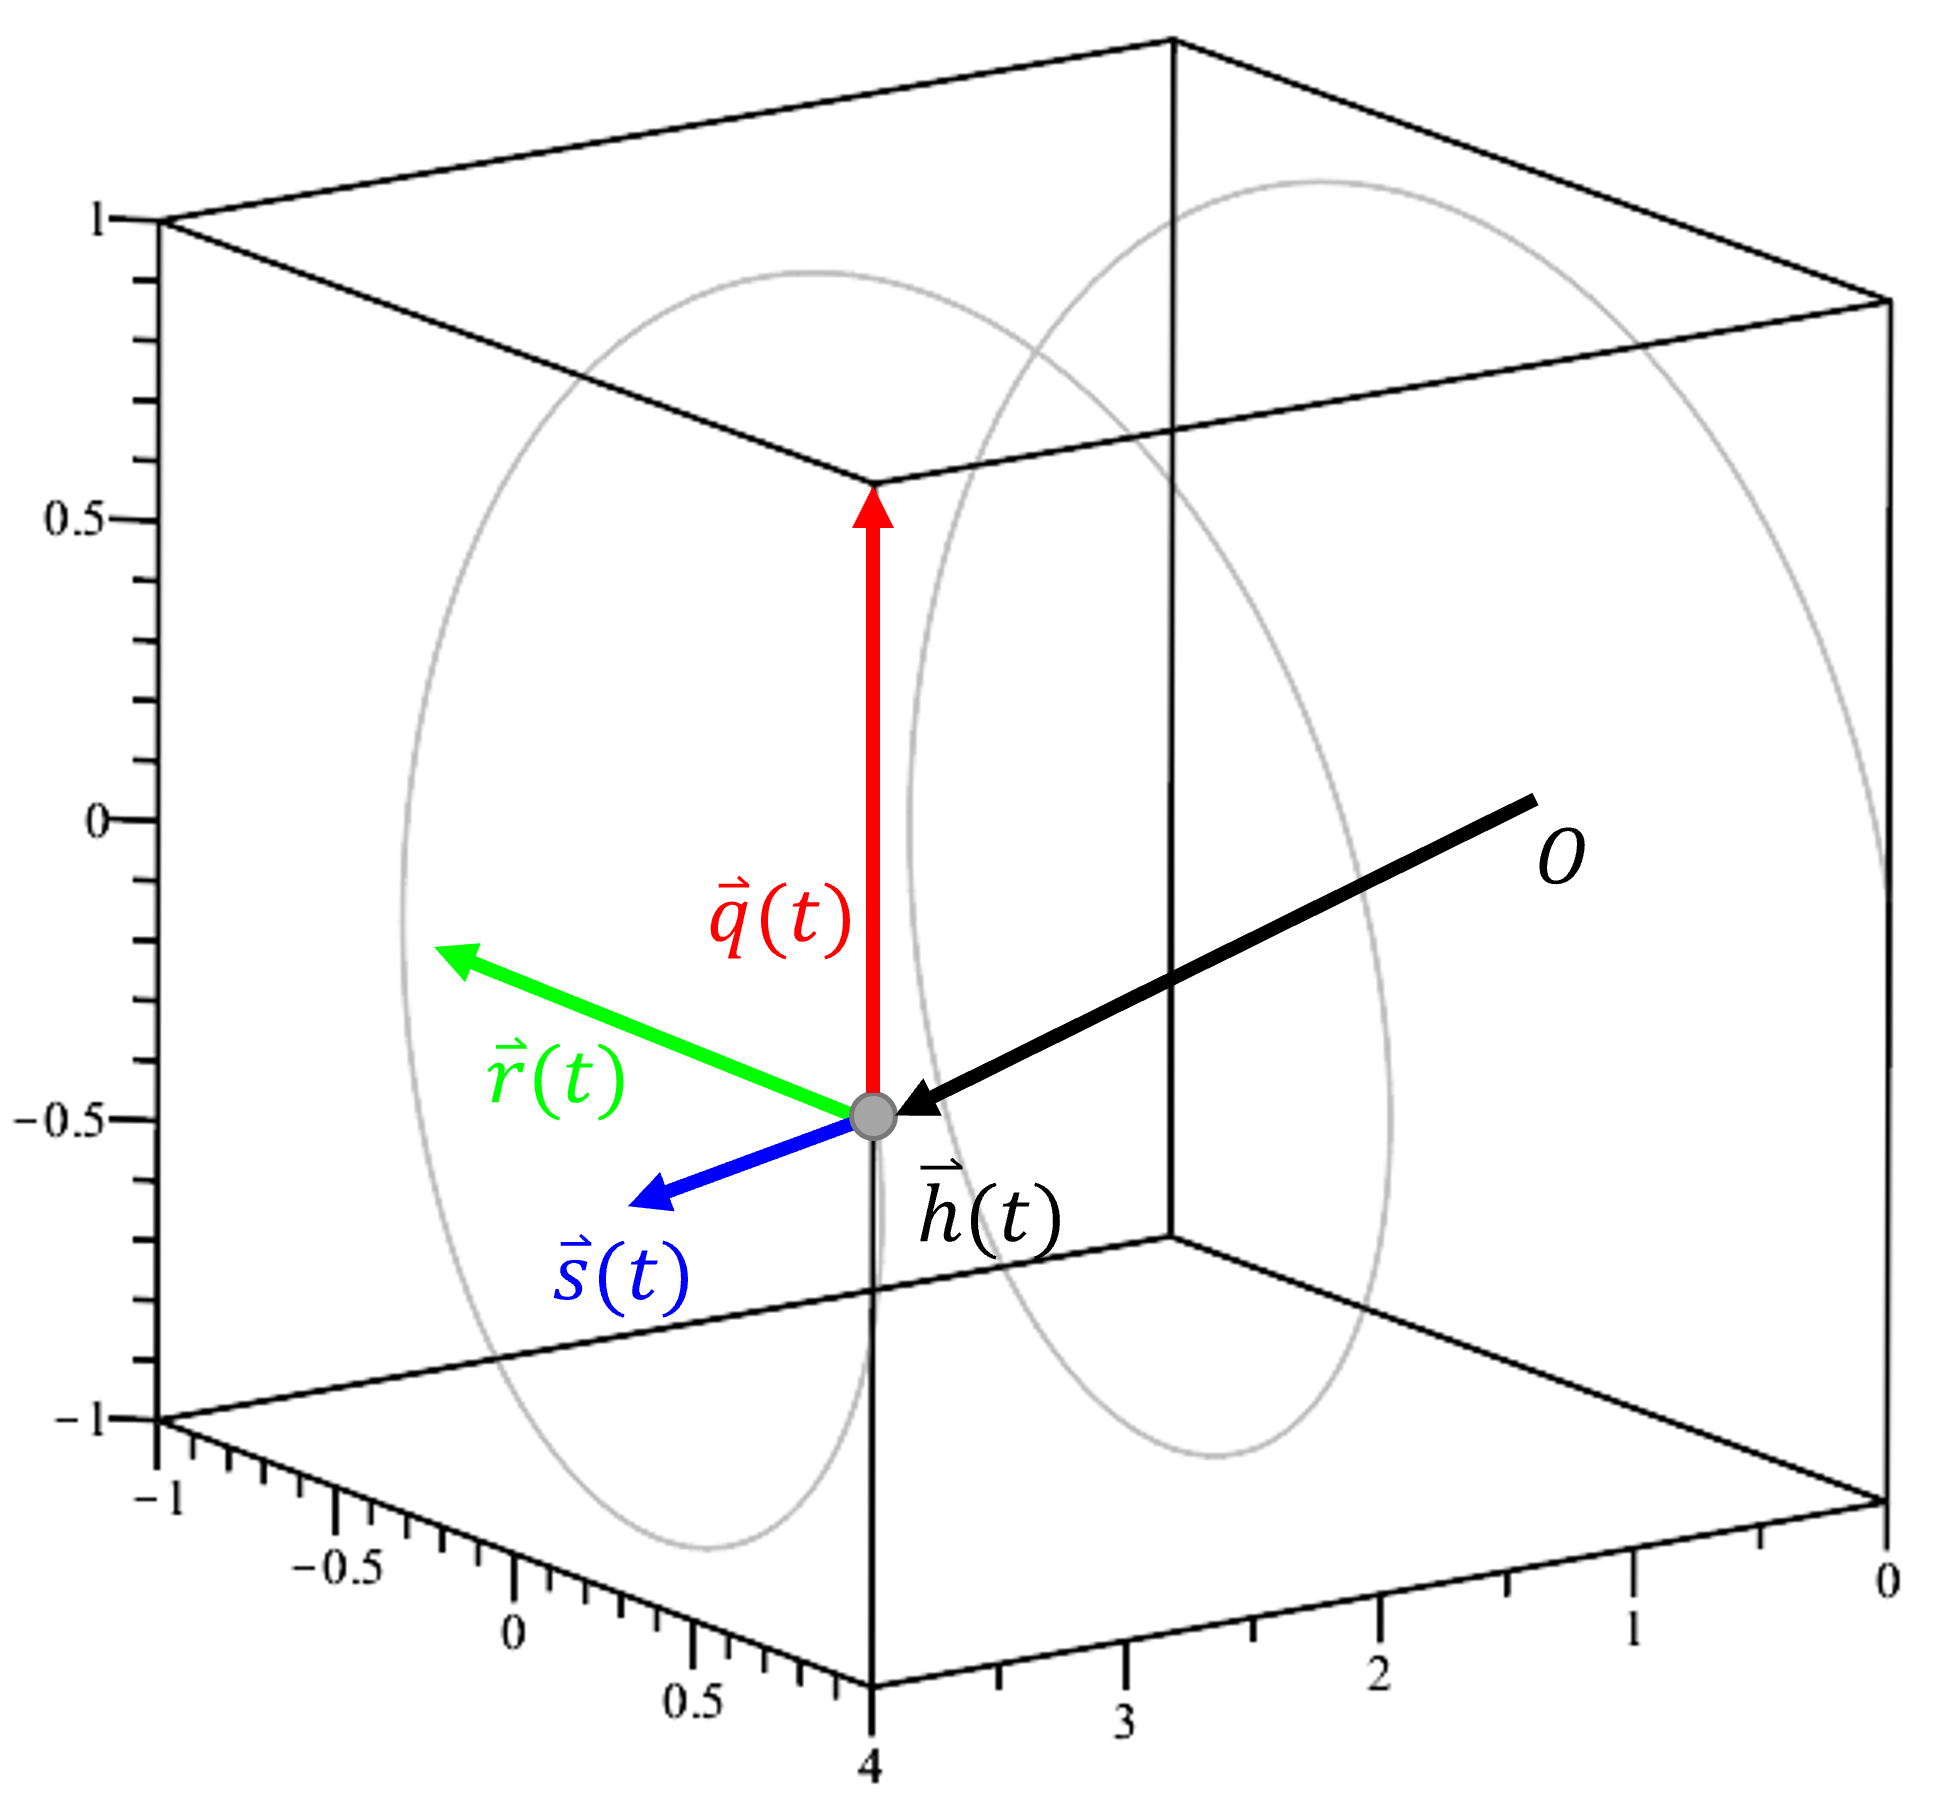
\includegraphics[width=\textwidth]{HelicalPath_r1_p2_coord}
			\end{figure}
		\end{column}
	\end{columns}

	\footnotetext[1]{\href{https://math.stackexchange.com/a/461637/575146}{what's the equation of helix surface?}}
}

\frame
{
	\frametitle{Helical Coil with Volume: Revolving the Circle}
	\begin{columns}
		\begin{column}{0.7\textwidth}
			\begin{itemize}
				\item Draw a circle of radius $r_m$ along a plane spanned by $\vec{r}(t)$ and $\vec{s}(t)$
				\item Introduce parameterization of the circle with variable $u$
				\item Convert into $(x,y,z)$ coordinates of the helical reference frame
				\item Add in parameter $\theta$ to control the starting rotational position
			\end{itemize}
		\end{column}
		\begin{column}{0.3\textwidth}
			\begin{figure}
				\centering
				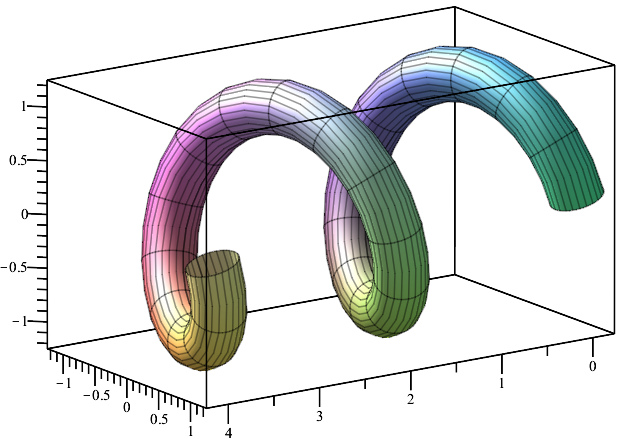
\includegraphics[width=0.8\textwidth]{HelicalCoil_r1_p2}
			\end{figure}
		\end{column}
	\end{columns}
	
	\begin{equation}
		\vec{H}(t,u) = \overbrace{\vec{h}(t)}^{\mathrm{helix}} + \overbrace{r_m\vec{r}(t)\cos(u) + r_m\vec{s}(t)\sin(u)}^{\textrm{circle}} \quad t=0,\ldots,2\pi\cdot n \quad u=0,\ldots,2\pi
	\end{equation}
	\begin{block}{Parameterized helical coil}
		\begin{equation}
			\vec{H}(t,u)=
			\begin{cases}
				x(t,u) = \frac{p}{2\pi}t+\frac{r_Mr_m\sin(u)}{\sqrt{r_M^2+\left(\frac{p}{2\pi}\right)^2}} \\
				y(t,u) = r_M\cos(t+\theta) - r_m\cos(t+\theta)\cos(u) + \frac{p\cdot r_m\sin(t+\theta)\sin(u)}{2\pi\sqrt{r_M^2+\left(\frac{p}{2\pi}\right)^2}} \\
				z(t,u) = r_M\sin(t+\theta) - r_m\sin(t+\theta)\cos(u) - \frac{p\cdot r_m\cos(t+\theta)\sin(u)}{2\pi\sqrt{r_M^2+\left(\frac{p}{2\pi}\right)^2}}
			\end{cases}
		\end{equation}
	\end{block}
} 

\frame
{
	\frametitle{Behaviour at Endpoints}
	\begin{columns}
		\begin{column}{0.7\textwidth}
			\begin{itemize}
				\item At zero strain ($\varepsilon=0$) the following holds:
			\end{itemize}
			\begin{table}
				\begin{tabular}{l c c}
					\toprule
					& \textbf{Wire} & \textbf{Elastic} \\
					\midrule
					$D$ & $d_w$ & $d_e(0)$ \\
					$l$ & $n\sqrt{\left(\pi(d_w+d_e(0))\right)^2+p^2}$ & $l$ \\
					$r_m$ & $\frac{1}{2}d_w$ & $\frac{1}{2}d_e(0)$ \\
					$r_M$ & $\frac{1}{2}(d_w+d_e(0))$ & $0$ \\
					\bottomrule
				\end{tabular}
			\end{table}
		\end{column}
		\begin{column}{0.3\textwidth}
			\begin{figure}
				\centering
				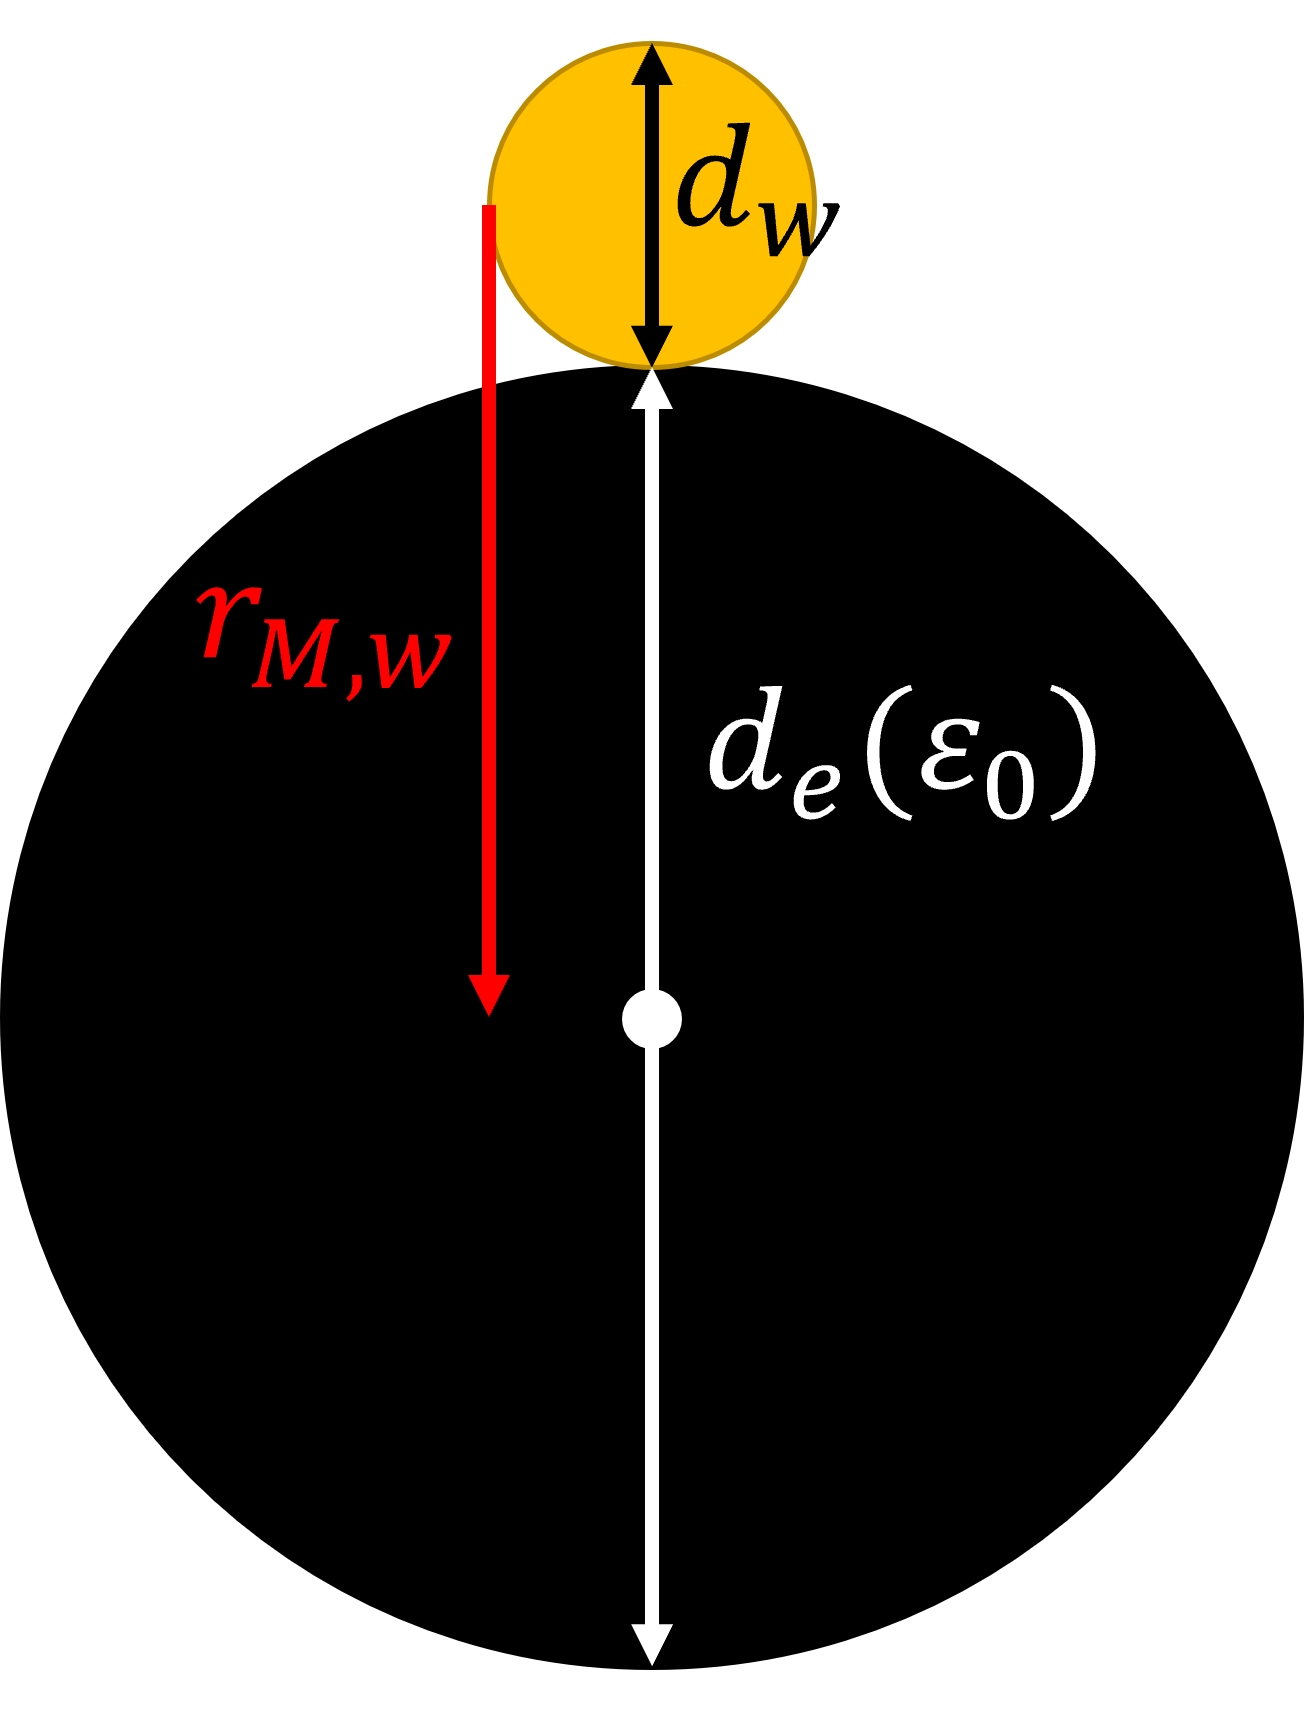
\includegraphics[width=0.6\textwidth]{UnstrainedCS}
			\end{figure}
		\end{column}
	\end{columns}
	\begin{columns}
		\begin{column}{0.7\textwidth}
			\begin{itemize}
				\item At the maximum strain ($\varepsilon_{max}$), the following holds:
			\end{itemize}
			\begin{table}
				\begin{tabular}{l c c}
					\toprule
					& \textbf{Wire} & \textbf{Elastic} \\
					\midrule
					$d$ & $d_w$ & \textcolor{OrangeRed}{$d_e(\varepsilon_{max})$} \\
					$l$ & $n\sqrt{\left(\pi(d_w+d_e(0))\right)^2+p^2}$ & \textcolor{OrangeRed}{$\star$} \\
					$r_m$ & $\frac{1}{2}d_w$ & $\frac{1}{2}\textcolor{OrangeRed}{d_e(\varepsilon_{max})}$ \\
					$r_M$ & $0$ & $\frac{1}{2}(d_w+\textcolor{OrangeRed}{d_e(\varepsilon_{max})})$ \\
					\bottomrule
				\end{tabular}
			\end{table}
		\end{column}
		\begin{column}{0.3\textwidth}
			\begin{figure}
				\centering
				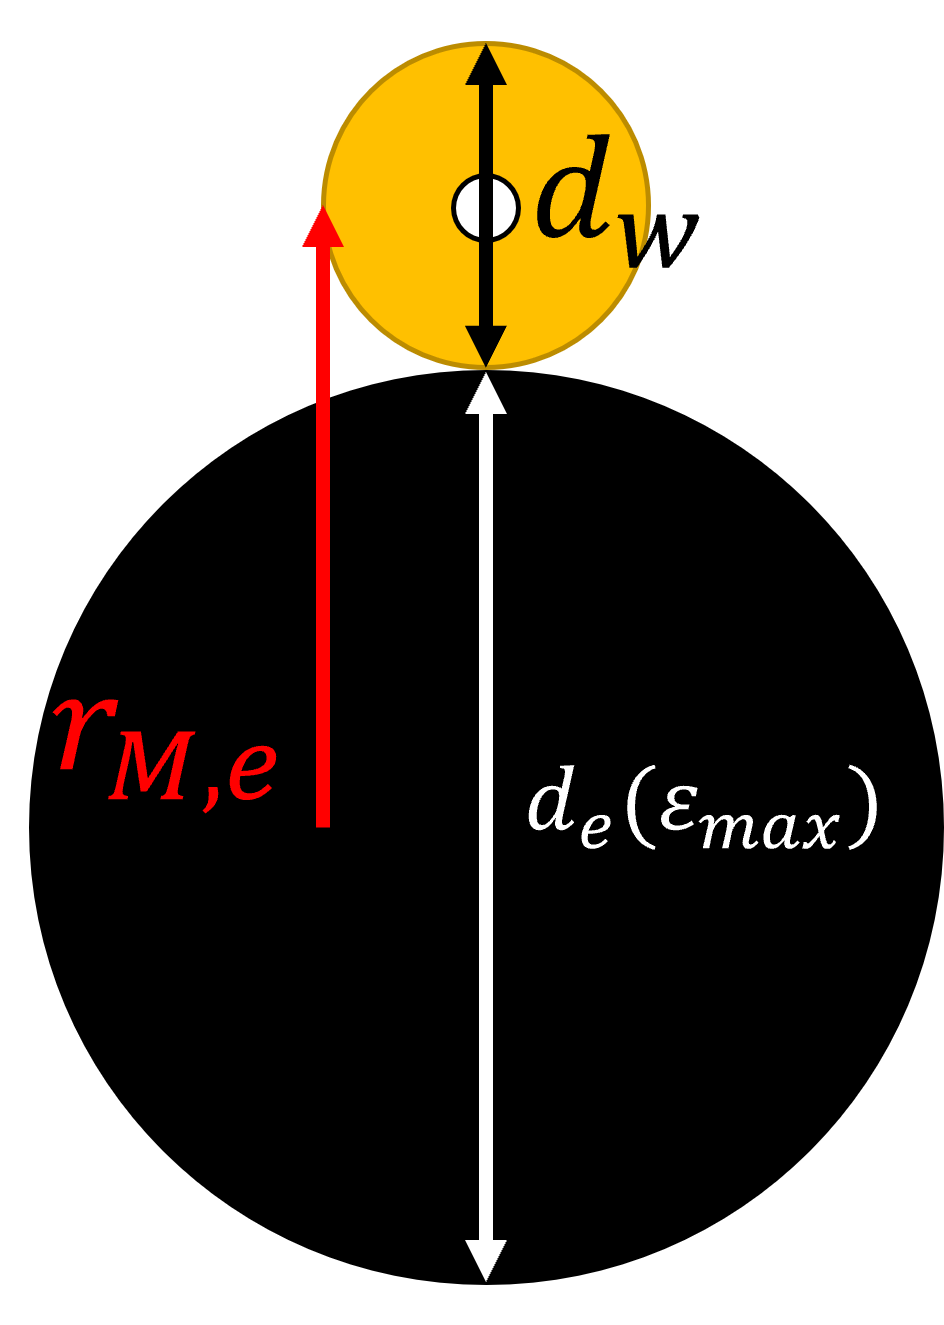
\includegraphics[width=0.4574\textwidth]{MaxstrainedCS}
			\end{figure}
		\end{column}
	\end{columns}
}

\frame
{
	\frametitle{Geometry of the Wire Coil}
	\begin{itemize}
		\item The wire helix minor radius is constant and its major radius is only dependent on initial conditions and strain $\varepsilon$.
		\item The wire does not stretch, so we can produce an equality to solve for its $r_M$ as a function of $\varepsilon$.
		\item Use the fact that changes linearly with strain $p(\varepsilon)=p(0)(1+\varepsilon)$.
	\end{itemize}
	\begin{align}
		l_w(0) &= l_w(\varepsilon) \nonumber \\
		n\sqrt{\left(\pi(d_w+d_e(0))\right)^2+p^2} &= n\sqrt{(\pi (2 r_{M,w}(\varepsilon)))^2 + (p(1+\varepsilon))^2} \nonumber \\
		r_{M,w}(\varepsilon) &= \frac{1}{2\pi}\sqrt{\pi^2(d_e(0)+d_w(0))^2 - p^2\varepsilon(\varepsilon+2)}
	\end{align}
	\begin{itemize}
		\item From these, the geometry of the wire coil $(r_M, r_m, p)$ at any strain is exactly defined.
		\item What about the elastic coil?
	\end{itemize}
}

\frame
{
	\frametitle{Constraints between Elastic and Wire}
	\begin{columns}
		\begin{column}{0.7\textwidth}
			\begin{itemize}
				\item The axis of the helices shifts from the centre of the elastic at $\varepsilon=0$ to the centre of the wire at $\varepsilon_{max}$ following:
			\end{itemize}
			\begin{equation}
				r_{M,e}(\varepsilon)=\frac{1}{2}\left(\textcolor{OrangeRed}{d_e(\varepsilon)}+d_w\right)-r_{M,w}(\varepsilon)
			\end{equation}
			\vspace{-1.5em}
			\begin{itemize}
				\item We now know expressions for $(r_M, r_m, p)$ of the elastic coil at arbitrary strain, but they are all dependent on the elastic diameter \textcolor{OrangeRed}{$d_e(\varepsilon)$}.
				\item Two equations can be written for the elastic length $l_e(\varepsilon)$:
				\begin{enumerate}
					\item Length from helical path: $l_{e,h}(\varepsilon) = f(\textcolor{OrangeRed}{d_e(\varepsilon)}, \varepsilon)$
					\item Length from Poisson's ratio: $l_{e,\nu}(\varepsilon) = f(\textcolor{OrangeRed}{d_e(\varepsilon)})$
				\end{enumerate}
				\item Can equate $l_{e,h}(\varepsilon) = l_{e,\nu}(\varepsilon)$ and solve for $d_e(\varepsilon)$ numerically.
			\end{itemize}
		\end{column}
		\begin{column}{0.3\textwidth}
			\begin{figure}
				\centering
				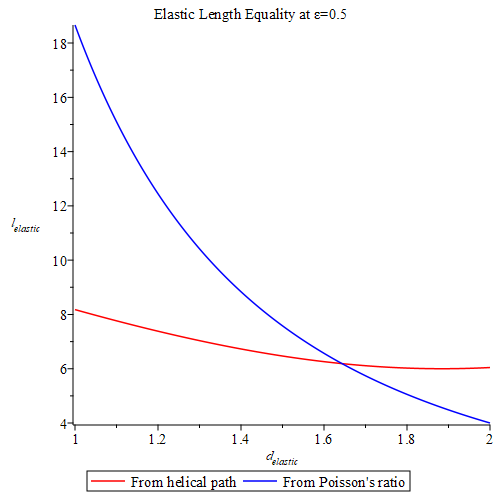
\includegraphics[width=\textwidth]{ElasticLengthEquality}
			\end{figure}
		\end{column}
	\end{columns}
	\begin{columns}
		\begin{column}{0.7\textwidth}
			\begin{block}{From Helical Path}
				\begin{minipage}[c][0.18\textheight][c]{\linewidth} 
				\begin{equation}
					\resizebox{\textwidth}{!}{$
						l_{e,h}(\varepsilon) = n\sqrt{4\pi^2\left(\frac{d_e(\varepsilon)+d_w}{2} - \frac{1}{2\pi}\sqrt{(d_e(0)+d_w)^2\pi^2-p^2\varepsilon(\varepsilon+2)}\right)^2+p^2(1+\varepsilon)^2}
					$}
				\end{equation}
				\end{minipage}
			\end{block}
		\end{column}
		\begin{column}{0.3\textwidth}
			\begin{block}{From Poisson's Ratio}
				\begin{minipage}[c][0.18\textheight][c]{\linewidth} 
				\begin{equation}
					\resizebox{\textwidth}{!}{$
						l_{e,\nu}(\varepsilon) = \exp{\left(-\frac{\ln\left(\frac{d_e(\varepsilon)}{d_e(0)}\right)}{\nu}\right)}l_0
					$}
				\end{equation}
				\end{minipage}
			\end{block}
		\end{column}
	\end{columns}
}

\frame
{
	\frametitle{Final Geometrical Model}
	\begin{itemize}
		\item An example for a helical auxetic sensor with $d_e(0)=1$, $d_w=0.1$, $p(0)=2$, $\nu=0.45$.
	\end{itemize}
	\begin{center}
		\animategraphics[loop,controls,width=6cm]{10}{img/HAYFrames/frame_}{001}{198}
	\end{center}
}

\frame
{
	\frametitle{Slicing the Helices}
	\begin{itemize}
		\item Conveniently, we want cross-sections along the x-axis of the helix (in the zy-plane).
		\item If we get the x-component of $\vec{H}(t,u)$ and solve it for $t$, we can substitute it back into the other components and find the equation for the slice of $\vec{H}(t,u)$ with a plane at $x=0$.
		\item Repeat for both wire and elastic helices, and optionally for the wire core to delineate the dielectric layer.
	\end{itemize}
	\begin{columns}
		\begin{column}{0.5\textwidth}
			\begin{figure}
				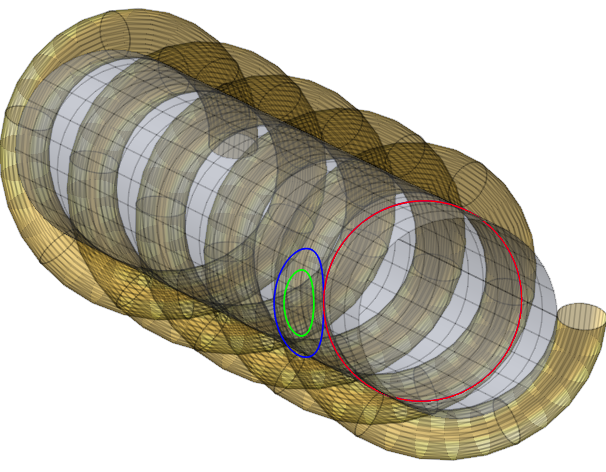
\includegraphics[width=0.6\textwidth]{SensorWithCS}
			\end{figure}
		\end{column}
		\begin{column}{0.5\textwidth}
			\begin{figure}
				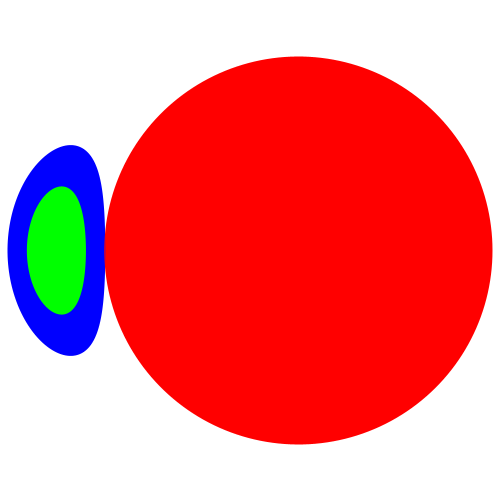
\includegraphics[width=0.6\textwidth]{SensorCS}
			\end{figure}
		\end{column}
	\end{columns}
}

\frame
{
	\frametitle{Calculating Capacitance}
	\begin{itemize}
		\item ATLC2\footnotemark: calculates transmission line parameters from cross-section.
		\item Multiply by length of strained sensor to estimate capacitance.
	\end{itemize}
	\begin{columns}
		\begin{column}{0.5\textwidth}
			\begin{figure}
				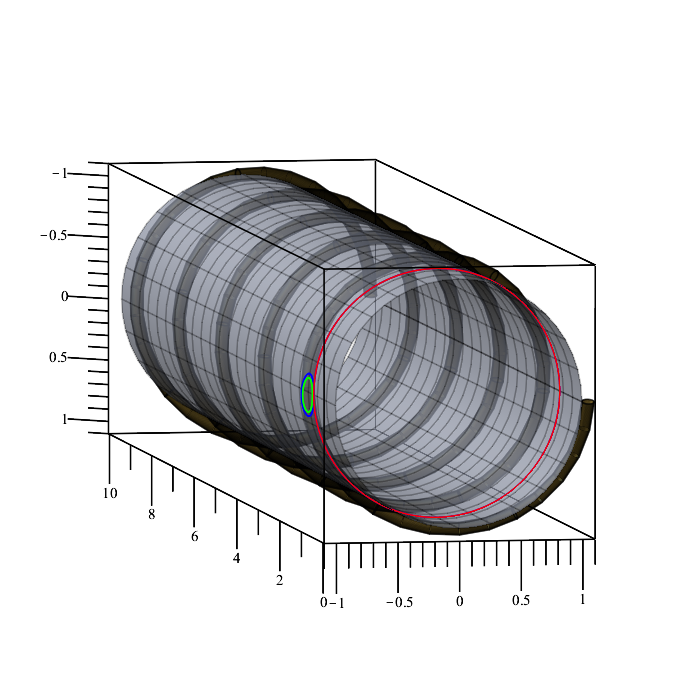
\includegraphics[width=0.5\textwidth]{helix_E3R1M_start_p2}
			\end{figure}
		\end{column}
		\begin{column}{0.5\textwidth}
			\begin{figure}
				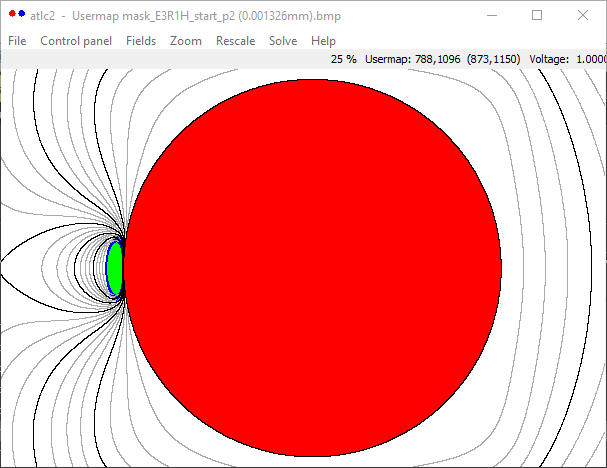
\includegraphics[width=0.5\textwidth]{field_E3R1M_start_p2}
			\end{figure}
		\end{column}
	\end{columns}
	\begin{columns}
		\begin{column}{0.5\textwidth}
		\end{column}
		\begin{column}{0.5\textwidth}
			\begin{figure}
				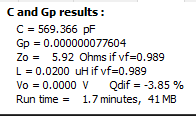
\includegraphics[scale=0.5]{ATLCResult}
			\end{figure}
		\end{column}
	\end{columns}
	\footnotetext{\href{http://www.hdtvprimer.com/kq6qv/atlc2.html}{Arbitrary Transmission Line Calculator}}
}

\end{document}
